% !TEX TS-program = pdflatex
% !TEX encoding = UTF-8 Unicode

% This is a simple template for a LaTeX document using the "article" class.
% See "book", "report", "letter" for other types of document.

\documentclass[11pt]{article} % use larger type; default would be 10pt

\usepackage[utf8]{inputenc} % set input encoding (not needed with XeLaTeX)
\usepackage{amsmath}
\usepackage{amssymb}
\usepackage{amsfonts}

%%% Examples of Article customizations
% These packages are optional, depending whether you want the features they provide.
% See the LaTeX Companion or other references for full information.

%%% PAGE DIMENSIONS
\usepackage{geometry} % to change the page dimensions
\geometry{a4paper} % or letterpaper (US) or a5paper or....
% \geometry{margin=2in} % for example, change the margins to 2 inches all round
% \geometry{landscape} % set up the page for landscape
%   read geometry.pdf for detailed page layout information

\usepackage{graphicx} % support the \includegraphics command and options

% \usepackage[parfill]{parskip} % Activate to begin paragraphs with an empty line rather than an indent

%%% PACKAGES
\usepackage{booktabs} % for much better looking tables
\usepackage{array} % for better arrays (eg matrices) in maths
\usepackage{paralist} % very flexible & customisable lists (eg. enumerate/itemize, etc.)
\usepackage{verbatim} % adds environment for commenting out blocks of text & for better verbatim
\usepackage{subfig} % make it possible to include more than one captioned figure/table in a single float
% These packages are all incorporated in the memoir class to one degree or another...

%%% HEADERS & FOOTERS
\usepackage{fancyhdr} % This should be set AFTER setting up the page geometry
\pagestyle{fancy} % options: empty , plain , fancy
\renewcommand{\headrulewidth}{0pt} % customise the layout...
\lhead{}\chead{}\rhead{}
\lfoot{}\cfoot{\thepage}\rfoot{}

%%% SECTION TITLE APPEARANCE
\usepackage{sectsty}
\allsectionsfont{\sffamily\mdseries\upshape} % (See the fntguide.pdf for font help)
% (This matches ConTeXt defaults)

%%% ToC (table of contents) APPEARANCE
\usepackage[nottoc,notlof,notlot]{tocbibind} % Put the bibliography in the ToC
\usepackage[titles,subfigure]{tocloft} % Alter the style of the Table of Contents
\renewcommand{\cftsecfont}{\rmfamily\mdseries\upshape}
\renewcommand{\cftsecpagefont}{\rmfamily\mdseries\upshape} % No bold!

%%% END Article customizations

%%% The "real" document content comes below...

\title{Computational Stochastic Processes - Assignment 1}
\author{Tom McGrath}
%\date{} % Activate to display a given date or no date (if empty),
         % otherwise the current date is printed 

\begin{document}
\maketitle

\section{Question 1}

\subsection{q1.a.}

Monte Carlo estimate with 100,000 samples: $Z = 4.2966847565923385e+19$

\subsection{q1.b.}
Numerical integration gives $Z = 4.667589495153099e+19$
Graph of error (blue) and variance (green) for MC integration:

\begin{figure}[h!]
	\centering
		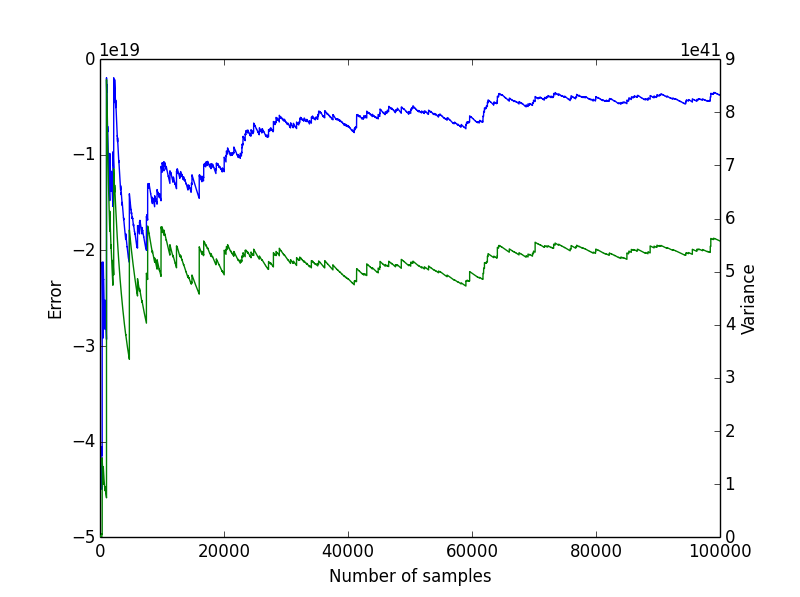
\includegraphics[scale = 0.5]{MC_err_var.png}
\end{figure}

\newpage

\subsection{q1.c}
Over $[-1,1] \times [-1,1]$, $f(x,y)$ looks like:

\begin{figure}[h!]
	\centering
		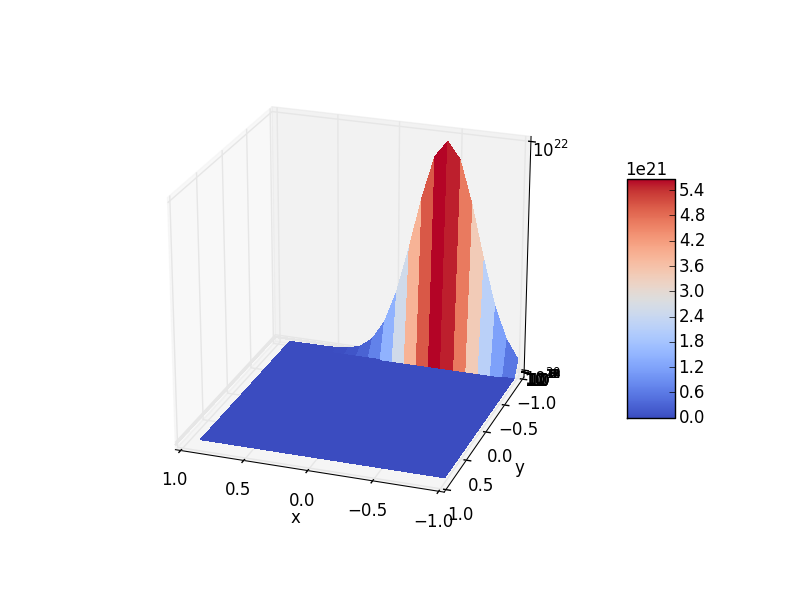
\includegraphics[scale = 0.5]{V_surface.png}
\end{figure}

There is another peak around $(0.5, 1)$, but it is smaller. A mixture of Gaussians is the appropriate distribution for importance sampling. The error \& variance performance is in the figure below:

\begin{figure}[h!]
	\centering
		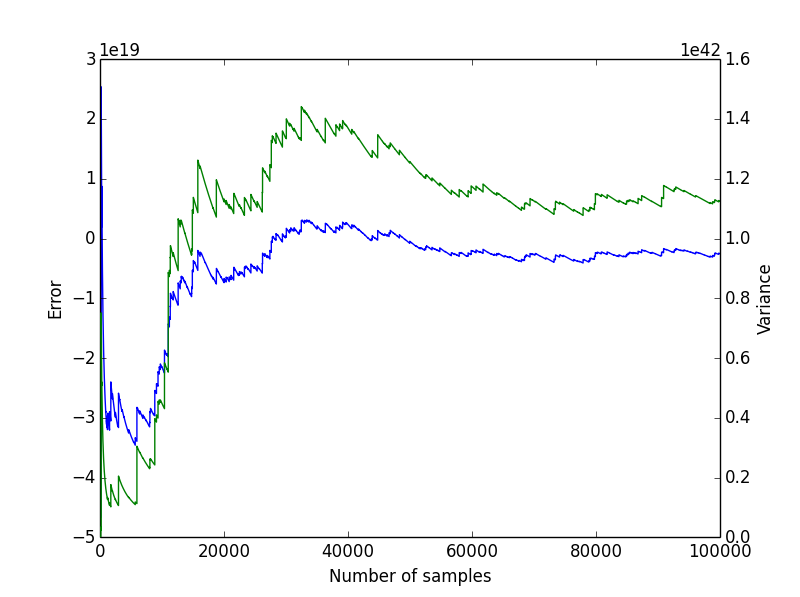
\includegraphics[scale = 0.5]{IS_err_var.png}
\end{figure}

\section{Question 2}
\subsection{q2.a.}
Generated sample paths and first four moments plotted below (mean is black, variance blue, 3rd moment green and 4th moment red):

\begin{figure}
	\centering
		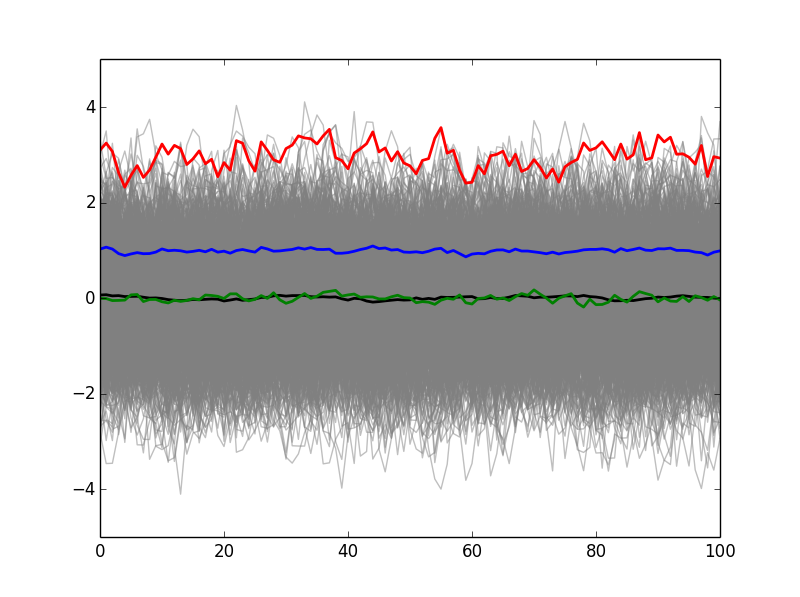
\includegraphics[scale = 0.5]{q2a.png}
\end{figure}

Odd moments are zero, as we would expect.

Mean square displacement graph:

\begin{figure}[h!]
	\centering
		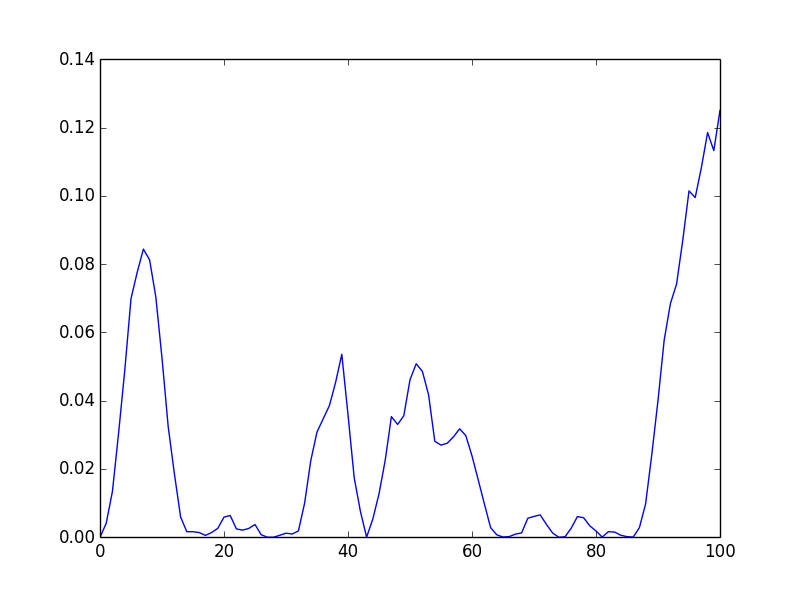
\includegraphics{q2rms.png}
\end{figure}

\subsection{q2.b.}
By Monte Carlo estimate with 100000 runs:

\begin{equation}
	\mathbb{P}\left( sup_{t \in [0,2]} X(t) > 2 \right) = 0.48992
\end{equation}

\section{Q3}
\subsection{q3.a.}

\begin{equation}
	dX(t) = \mu(t)dt + \Sigma(t)dW(t), \quad X(0) = x
\end{equation}

Integrating we obtain:

\begin{equation}
	X(t) = X(0) + \int^{t}_{0}\mu(s)ds + \int^{t}_{0}\Sigma(s)dW(s)
\end{equation}

We have to deal with the integral with respect to $W(s)$ - this is a martingale with quadratic variation:

\begin{equation}
	I(t) = \int^{t}_{0}\Sigma(s)ds \implies \langle I(t) \rangle = \int^{t}_{0}(\Sigma(s) \otimes \Sigma(s))ds = \int^{t}_{0}\Gamma(s)ds
\end{equation}

Therefore we have:

\begin{equation}
	X(t) = X(0) + \int^{t}_{0}\mu(s)ds + \int^{t}_{0}\Gamma(s)ds
\end{equation}

The characteristic function of a random variable $X$ is given by:

\begin{equation}
	\phi(t) = \mathbb{E}(e^{itX})
\end{equation}

Which is Gaussian when:

\begin{equation}
	\phi(t) = e^{\langle m, t\rangle - \frac{1}{2}\langle t, \Sigma t\rangle}
\end{equation}

The $X(t)$ determined above satisfies this, and the equation for $X(t) - X(s)$ follows immediately.

\subsection{q3.b.}
By discretising time and calculating increments according to equation $(4)$ on the problem sheet it is possible to generate sample paths for $X(t)$.

\subsection{q3.c.}
Figure of sample path (x component in blue, y component in green):

\begin{figure}
	\centering
		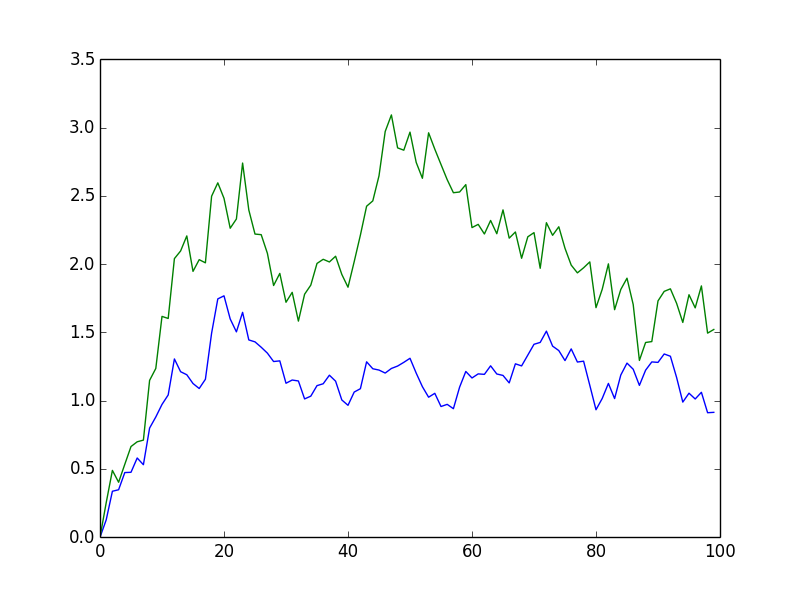
\includegraphics[scale = 0.5]{q3c.png}
\end{figure}

Figure of mean and variance:
\begin{figure}[h!]
	\centering
		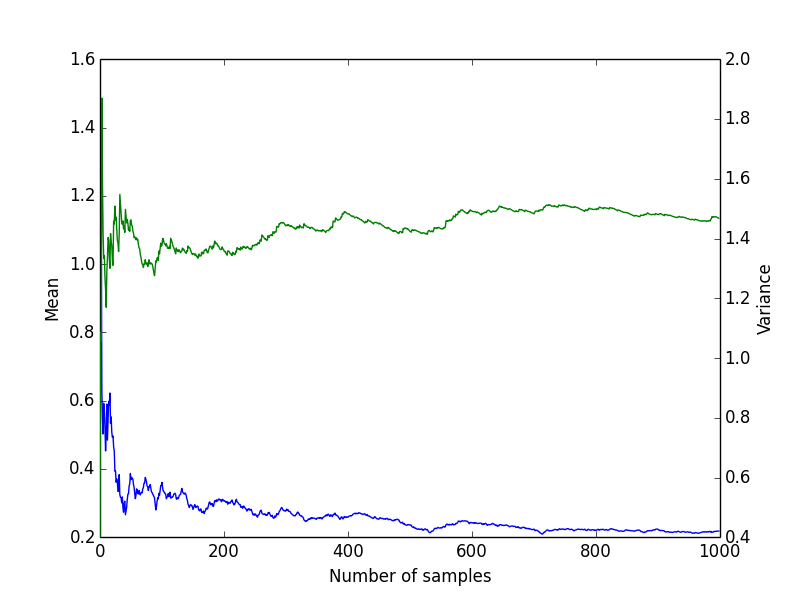
\includegraphics[scale = 0.5]{q3c2.png}
\end{figure}

Figure of elements of covariance matrix:
\begin{figure}[h!]
	\centering
		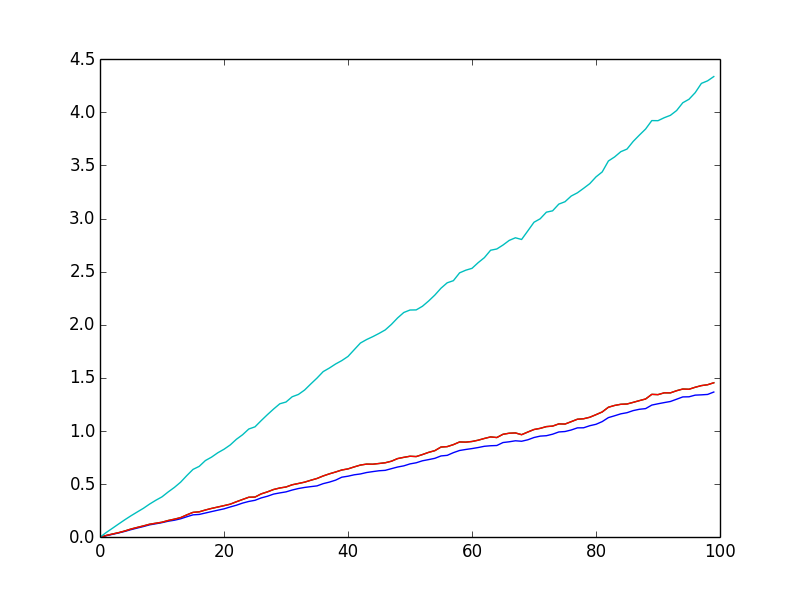
\includegraphics[scale = 0.5]{q3c3.png}
\end{figure}

The results match theoretical predictions well. Even with a relatively low number of sample paths, a good agreement is still occurring.

\section{Q4}
\subsection{q4.a.}
Using code from question 2 with the covariance function provided it is possible to generate samples from this field. Samples and first 4 moments are plotted below:

\begin{figure}[h!]
	\centering
		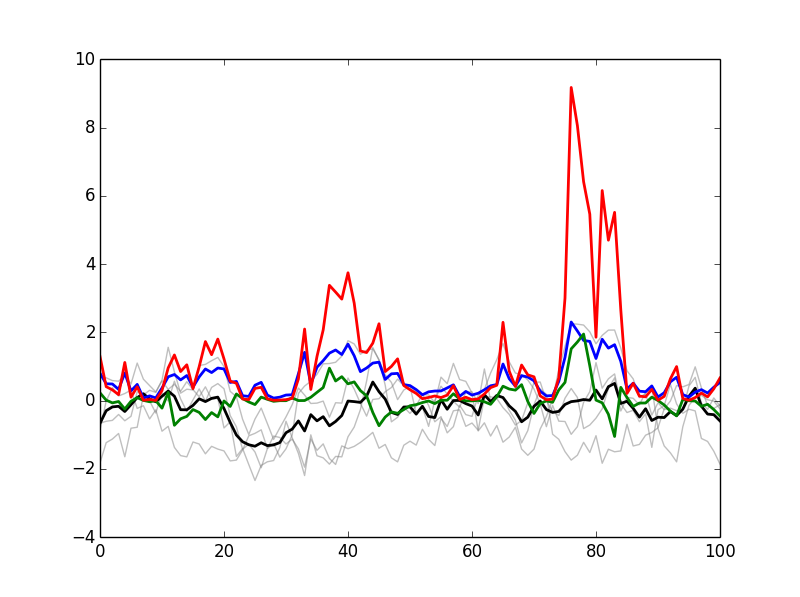
\includegraphics[scale = 0.5]{q4a2.png}
\end{figure}

For 1000 samples, the first 4 moments are:
\begin{figure}[h!]
	\centering
		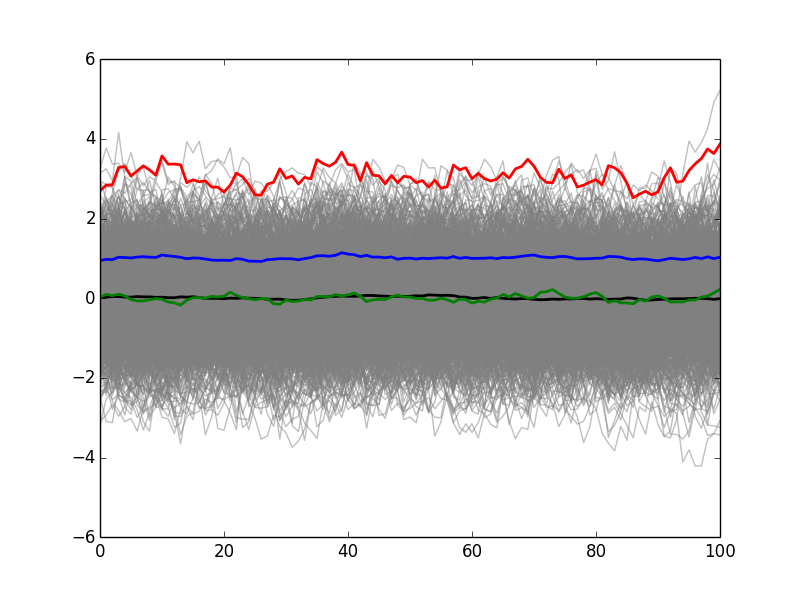
\includegraphics[scale = 0.5]{q4a.png}
\end{figure}

\subsection{q4.b.}
We have that:

\begin{equation}
	\int^{L}_{-L}e^{-a|x-y|}f(y)dy = \lambda f(x)
\end{equation}

Which is equivalent to

\begin{equation}
	\int^{x}_{-L}e^{-a(x-y)}f(y)dy + \int^{L}_{x}e^{a(x-y)}f(y)dy = \lambda f(x)
\end{equation}

Differentiating once with respect to t gives:
\begin{equation}
	-a\int^{x}_{-L}e^{-a(x-y)}f(y)dy + a\int^{L}_{x}e^{a(x-y)}f(y)dy - e^{-ax}e^{ax} + e^{-ax}e^{ax} = \lambda f'(x)
\end{equation}

The last 2 terms cancel. Differentiating again gives:

\begin{equation}
	a^{2}\int^{x}_{-L}e^{-a(x-y)}f(y)dy + a^{2}\int^{L}_{x}e^{a(x-y)}f(y)dy - 2af(x)  = \lambda f''(x)
\end{equation}

The terms in $a^{2}$ are now the original integral multiplied by a factor of $a^{2}$, so we can write:

\begin{equation}
	a^{2}\lambda f(x) - 2af(x) = \lambda f''(x)
\end{equation}

We can obtain the boundary conditions by evaluating the undifferentiated expression and the first derivative at the boundaries $+L$ and $-L$ to give:

\begin{align}
a f(L) &+ f'(L) = 0\\
a f(-L) &- f'(-L) = 0
\end{align}

Now use the variation of constants method, with eigenfunctions in the form:

\begin{equation}
f(x) = c_{1} \cos(\omega x) + c_{2} \sin(\omega x)
\end{equation}

Firstly we can recover the eigenvalues:

\begin{equation}
	a^{2}\lambda f(x) - 2af(x) = \lambda f''(x) \implies a^{2}\lambda f(x) + 2 a f(x) = \omega^{2}\lambda f(x)
\end{equation}

Rearranging gives:

\begin{equation}
	(a^{2} = \omega^{2})\lambda = 2a \implies \lambda = \frac{2a}{a^{2} + \omega^{2}}
\end{equation}

Now inserting the eigenfunctions and their derivatives into the boundary conditions gives the following equations:

\begin{align}
	&c_{1}(a - \omega \tan(\omega L)) + c_{2}(\omega + a \tan(\omega L)) = 0\\
	&c_{1}(a - \omega \tan(\omega L)) - c_{2}(\omega + a \tan(\omega L)) = 0
\end{align}

These have nontrivial solutions when either the term in $c{1}$ or the term in $c_{2}$ is zero, and gives solutions:

\begin{equation}
	f(x) = \frac{\cos(\omega x)}{\sqrt{L + \frac{\sin(2\omega L)}{2\omega}}}
\end{equation}

for the solutions given by $a - \omega \tan(\omega L) = 0$ and

\begin{equation}
	f(x) = \frac{\sin(\omega x)}{\sqrt{L - \frac{\sin(2\omega L)}{2\omega}}}
\end{equation}

for solutions given by $\omega + a \tan(\omega L) = L$

\end{document}
